\documentclass[11pt,a4paper]{article}
\usepackage[hyperref]{acl2018}
\usepackage{times}
\usepackage{latexsym}
\usepackage{graphicx}
\usepackage{url}

\aclfinalcopy % Uncomment this line for the final submission
%\def\aclpaperid{***} %  Enter the acl Paper ID here

%\setlength\titlebox{5cm}
% You can expand the titlebox if you need extra space
% to show all the authors. Please do not make the titlebox
% smaller than 5cm (the original size); we will check this
% in the camera-ready version and ask you to change it back.

\newcommand\BibTeX{B{\sc ib}\TeX}

\title{Parsing Database Queries in Natural Languages: A Purely Empirical Method}

\author{Li, Ziyao \\
  1500017776 / Yuanpei College \\
  {\tt leeeezy@pku.edu.cn}
  }

\date{}

\begin{document}
\maketitle
\begin{abstract}
  This paper is the Project 2 of \textit{Course EMNLP}. The main task is to realize a model to parse given database queries, which are in natural language forms, to an operable form. Literally, the given parser form do have a lot of differences than the first-order logic (FOL) forms. The model leveraged several hand-crafted rules according to the observations of the data and an Inductive Logic Programming framework proposed in CHILL \footnote{Zelle, J. M. and R. J. Moorey, Learning to Parse Database Queries Using Inductive Logic Programming, In \textit{Proceedings of the Thirteenth National Conference on Artificial Intelligence (AAAI)}, Aug 1996}. Rules for different predicates are come up with, as well as several language phenomena are encoded. A $47.48\%$ \textit{Exact Accuracy}, as demanded by the project, over database \texttt{geo800} was achieved.
\end{abstract}

\section{Introduction - Datasets and Problem Definition}

Instead of a semantic parsing project, the data provided in this project is more like a down-stream Question-Answering task. A functional form of data is provided instead of the $\lambda$-calculus formulas. Therefore, applying first-order logic (FOL)-based algorithms seems to be even more laborious, given the fact that all these algorithms are sometimes artificially established and delicately elaborated, and that due to the complication of the system, the implementations of algorithms are not thoroughly described in short conference papers.

Figure 1 is an example of the query data. The annotated labels of instances are actually old-fashioned \textit{perl} codes. The $:-$ operator appearing in the data is inductions, or to say, clauses.  These induction examples, combined with a similarly defined database query language system and hundreds of control rules and basic induction rules, are directly used to transform a natural language sentence into a value (or a list of values) in the given database.

\begin{figure}[ht]
\vskip 0.2in
\label{fig1}
\begin{center}
\centerline{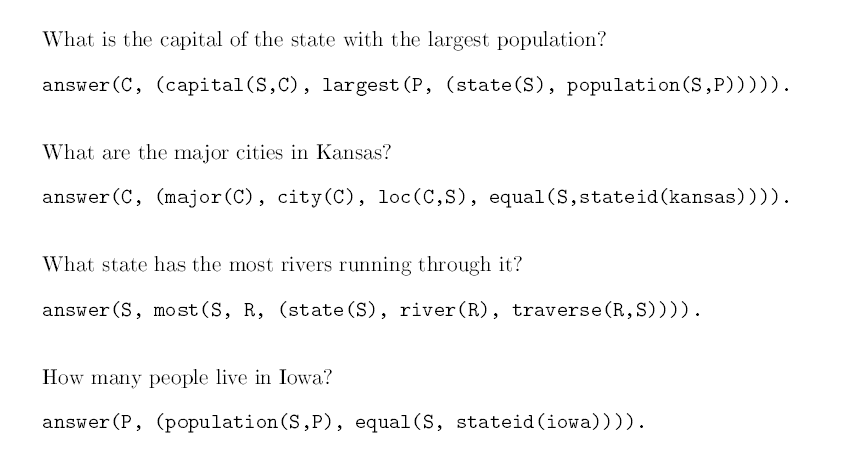
\includegraphics[width=\columnwidth]{fig1}}
\caption{An instance $(Input,Query)$, or $(parse,answer)$ pair of the data. A connection between the predicates in the language and the predicates in the logical form can be somehow inducted from a set of lexicon.}
\end{center}
\vskip -0.2in
\end{figure}

The original data and codes (the database and some of the complementary descriptions) are provided by Raymond J. Mooney from University of Texas, Austin \footnote{\url{ftp://ftp.cs.utexas.edu/pub/mooney/chillin/}}. To solve the problem defined above, an Induction Logical Programming (ILP)-based system was proposed in (J. Zelle \& R. Moorey, 1996)\footnote{Zelle, J. M. and R. J. Moorey, Learning to Parse Database Queries Using Inductive Logic Programming, In \textit{Proceedings of the Thirteenth National Conference on Artificial Intelligence (AAAI)}, Aug 1996}, along with a more detailed and descriptive illustration proposed in (J. Zelle \& R. Moorey, 1997)\footnote{Zelle, J. M. and R. J. Moorey, An Inductive Logic Programming Method for Corpus-based Parser Construction, Technical Report, 1997}.

\section{CHILL - Automatically Induction Rules Generator}

CHILL (Constructive Heuristics Induction for Language Learning) is still a rule-based system, while its rule-generation mechanism is not by human forces but by an induction framework elaborated according to the structure of the problem. Figure 2 shows the total structure of CHILL. The starting point of CHILL, however, is still a lexicon created manually of a mapping from natural language words to logical predicates.

\begin{figure}[ht]
\vskip 0.2in
\label{fig2}
\begin{center}
\centerline{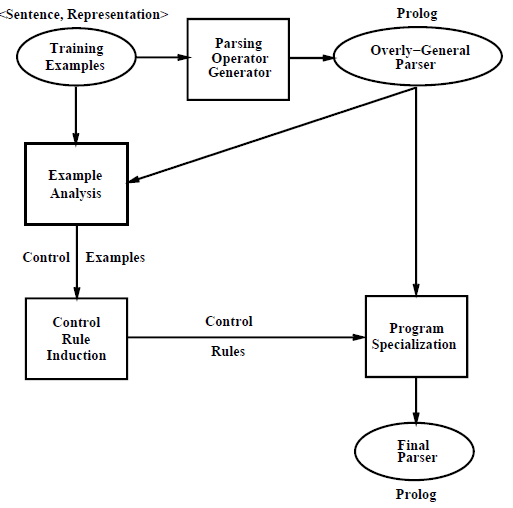
\includegraphics[width=\columnwidth]{fig2}}
\caption{A brief structure demonstration of CHILL.}
\end{center}
\vskip -0.2in
\end{figure}

\subsection{Parsing Framework}

The parsing framework defined in CHILL is perhaps the most ingenious part of the paper. The parsing process is considered as a sequential one incorporating the state-transformation of the parser stack and the sentence queue. Several basic operations can be defined over this framework. As for this database query parsing problem, five basic actions, namely \texttt{INTRODUCE}, \texttt{COREF\_VARS}, \texttt{SHIFT}, \texttt{LIFT\_CONJ} and \texttt{DROP\_CONJ} are defined.

\texttt{INTRODUCE} pushes a predicate onto the stack based on a word appearing in the input and information about its possible meanings in the lexicon. \texttt{COREF\_VARS} binds two arguments of two different predicates on the stack. \texttt{DROP\_CONJ} (or \texttt{LIFT\_CONJ}) takes a predicate on the stack and puts it into one of the arguments of a meta-predicate on the stack. \texttt{SHIFT} simply pushes a word from the input buffer onto the stack.

Figure 3 is an example to illustrate the whole process. This structure is the inspiration of the rule-based model proposed in this paper.

\begin{figure}[ht]
\vskip 0.2in
\label{fig3}
\begin{center}
\centerline{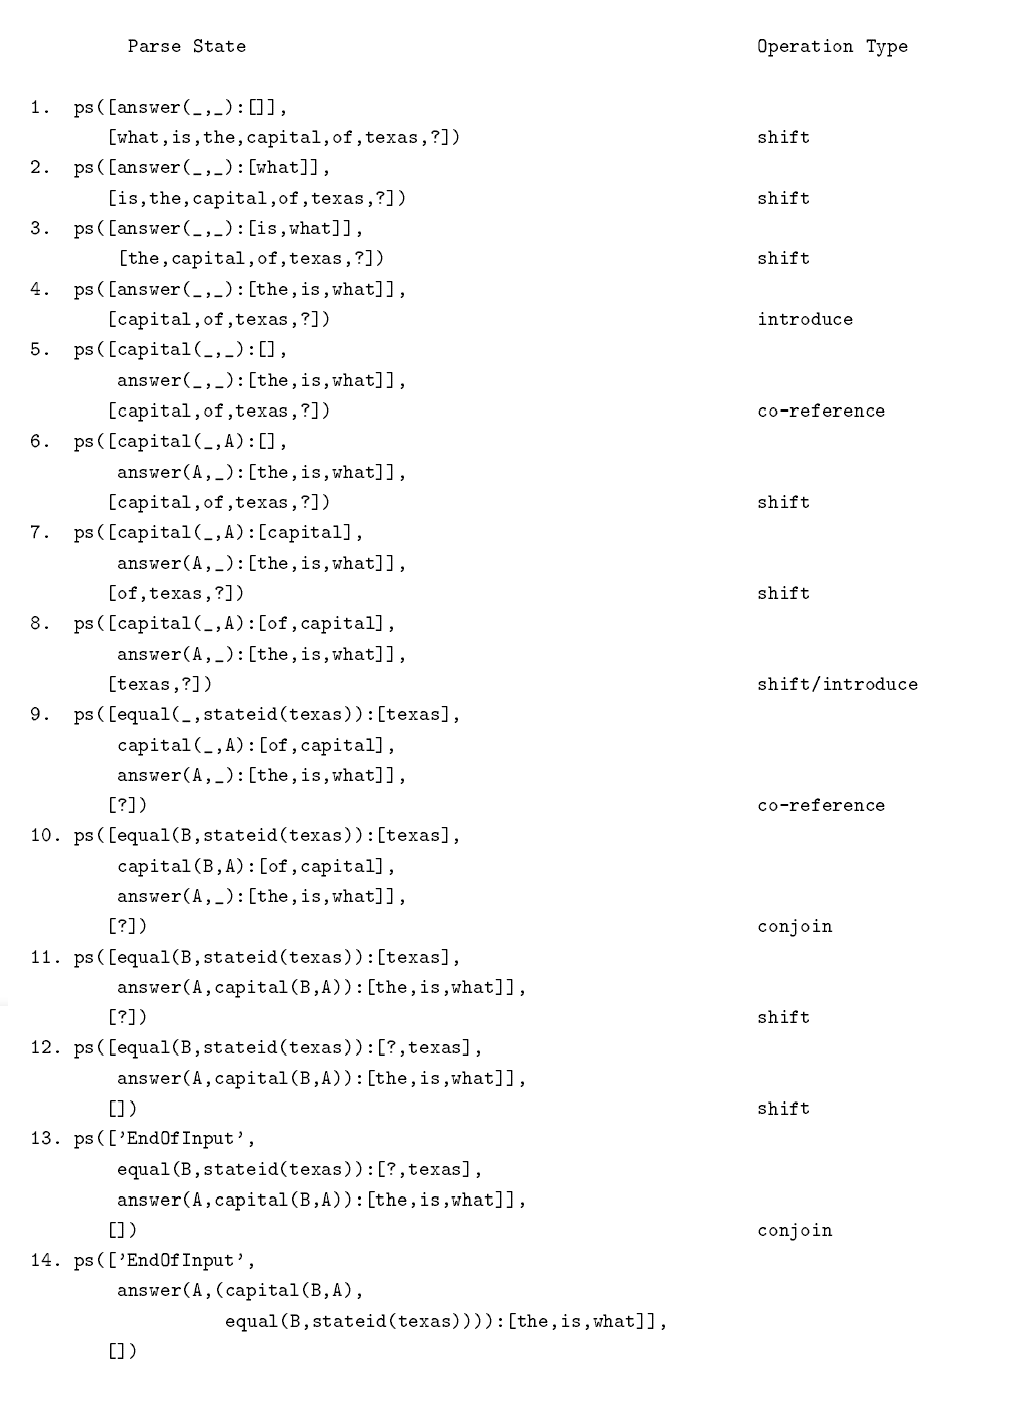
\includegraphics[width=\columnwidth]{fig3}}
\caption{An example of the parsing framework defined in CHILL.}
\end{center}
\vskip -0.2in
\end{figure}

\subsection{Example Analysis \& Induction Algorithms}

In this part, CHILL take into account all possible emerging actions and states as the data space, considering the emerged ones in the dataset as Positive examples and those do not the Negative. The idea is to find minimized generalizations to reduce the structure of the positive samples while in the same time avoiding introducing negative samples. A least generalize generalization (LGG) is evaluated in all pairs of positive samples while a generalization algorithm is proposed to conduct the induction process.

After control rules are inducted, a Program Specialization combines the rules and the basic induction rules into a unified output parser. On the dataset the derived parser is the most compacted without introducing negative samples.

\section{BroC Parser}

However, implementing the task is really hard, especially not using \textit{Perl} language (its powerful regular expression can save a lot of time). Therefore, by introducing several priors of the parsing framework we can have a easy-implementing algorithm - BroC Parser. The model is an \textit{ad hoc} taking into account a lot of background knowledge.

Here are the basic priors for the parser.
\begin{itemize}
  \item BroC Parser always \texttt{INTRODUCE} when the front of the sentence queue can be explained as a predicate in the lexicon.
  \item After \texttt{INTRODUCE}, BroC Parser always \texttt{SHIFT} all words used to \texttt{INTRODUCE} predicates. The shift process is simplified as a \texttt{pop} action.
  \item When \texttt{INTRODUCE} is not available, Broc Parser \texttt{SHIFT} one word from the sentence queue
  \item For each predicate, if it's a \textit{meta} one, directly \texttt{LIFT\_CONJ} it on the current mother \textit{meta} predicate, and regard it as the mother \textit{meta} predicate. If not, \texttt{LIFT\_CONJ} it on the back of the current mother \textit{meta} predicate. As \texttt{answer/2} is always the first predicate on the stack, reckon it as the first mother \textit{meta} predicate so the process can always going on.
  \item Small adjustments are made according to the train set.
\end{itemize}

The lexicon defined for the predicate-recognition task is trivial and not very interesting, so as the detailed adjustments made in the very \textit{ad hoc} project. The interested can take a look at the codes in \texttt{brocparser.py}.

\section{Experiments}

As the model is \textit{ad hoc} and take overwhelming differences over different datasets, only \texttt{geo880} dataset is experimented. As this is a rule-based system tuned on the train set, the precision over the train set is still a little bit higher than that over the validation set. Table 1 shows the result.

\begin{table}
\label{tab1}
\centering
\begin{tabular}{|l|r|}
\hline
Train & 0.5762 \\
\hline
Valid & 0.5444 \\
\hline
\end{tabular}
\caption{Exact Accuracy over \texttt{geo880} dataset.}
\end{table}

An \textit{Exact Accuracy} is examined as instructed by the project. However, taking such a measurement is unreasonable since the idea is never to produce identical logical forms by equivalent ones, ones that extract the same and therefore the correct responds to test queries. A great percentage of instances are provided with equivalent but different forms by the algorithm.

\section*{Appendix}

Some of the codes are written with Jupyter Notebook, but are all laborious and redundant work. Codes are in \texttt{bash.py}, \texttt{brocparser.py} and \texttt{structures.py}. \texttt{bash.py} implements a basic file reading and writing job. \texttt{brocparser.py} is the main parser and \texttt{structures.py} provides basic tool functions and data structures used in the other two codes. Besides, \texttt{d1\_train\_myout.txt}, \texttt{d1\_valid\_myout.txt} and \texttt{d1\_test\_myout.txt} are results provided from the algorithm.

It is future work to clean up some redundant work in the RuleParser class and to implement better APIs. Limited by the strong priors, some of the code cannot correctly parse the idea, but can be fixed by altering the \texttt{COREF\_VARS} principles, which should be easy to implement.


\end{document}
